
%!TEX ROOT=ctutest.tex

\chapter{Dynamický model}

Pro výpočet a predikci spotřeby elektrické energie je nezbytné vytvořit matematický dynamický model robota. 

V případě 6-ti osového manipulátoru se jedná o systém se šesti stupni volnosti. K popisu jeho dynamiky je proto potřeba 6 rovnic druhého řádu. Celkově se tedy jedná o systém dvanáctého řádu. 

\section{Pohybové rovnice}
\label{pohybove_rovnice_sec}
K odvození pohybových rovnic je možné použít jeden ze dvou základních přístupů a to Newton-Eulerovu metodu nebo Euler-Lagrangeovu metodu. 

Newton-Eulerova metoda je založena na přístupu k systému jako k soustavě jednotlivých jeho částí a vyžaduje určení pohybových rovnic každé jednotlivé osy. Protože jsou jednotlivé osy vzájemně kinematicky propojeny, jsou i pohybové rovnice jednotlivých os závislé na pohybu ostatních os. 

Euler-Lagrangeova metoda naopak přistupuje k systému jako k celku a je založena na určení Lagrangianu, který je definován jako rozdíl jeho celkové kinetické a potenciální energie. Dynamické rovnice systému se poté odvodí vypočtením Lagrangeových rovnic druhého druhu pro všechny stupně volnosti.

Oba přístupy nakonec vedou ke stejným rovnicím. Protože jsou jednotlivé polohy a dynamika systému popisovány pomocí úhlů na jednotlivých osách, jsou tyto rovnice silně nelineární. V případě robota KR5 se jedná o soustavu 6 rovnic o celkem 24 neznámých (moment, poloha, rychlost a zrychlení pro každou osu). 

Rovnice systému je možné zapsat v následujícím maticovém tvaru jako 

\begin{equation}
T = M(\dot{\theta},\theta)\ddot{\theta} + C(\dot{\theta},\theta)\dot{\theta} + G(\theta)
\label{dyn_rovnice_eq}
\end{equation}

kde

\begin{description}
\item[$T = {\big[T_1  \dotsm  T_n\big]}^{T}$] je vektor momentů sil působících na jednotlivé osy robota
\item[$\ddot \theta = {\big[\ddot \theta_1  \dotsm  \ddot \theta_n\big]}^{T}$] je vektor úhlových zrychlení na jednotlivých osách
\item[$\dot \theta = {\big[\dot \theta_1  \dotsm  \dot \theta_n\big]}^{T}$] je vektor úhlových rychlostí na jednotlivých osách
\item[$M\big(\dot \theta, \theta\big)$] je matice setrvačnosti tvořena tenzory setrvačnosti jednotlivých os
\item[$C\big(\dot \theta, \theta\big)$] je matice Coriolisových a odstředivých momentů sil působících na jednotlivé osy
\item[$G\big(\theta\big)$] je matice gravitačních sil působících na jednotlivé osy
\item[$n$] je počet os
\end{description}

K výpočtu okamžité spotřeby elektrické energie je nutné řešit inverzní dynamickou úlohu, kdy se z okamžitých poloh, rychlostí a zrychlení na jednotlivých osách robota vypočítají točivé momenty, kterými působí motory. 

Moment síly motoru je závislý na proudu protékajícím jeho vinutím. Tuto závislost je často možné aproximovat lineární závislostí a psát jako
\begin{equation}
T\big(t\big) = KI\big(t\big)
\label{torque_current_eq}
\end{equation}

kde

\begin{description}
\item[$T\big(t\big) {\big[Nm\big]}$] je moment síly motoru 
\item[$K {\big[Nm/A\big]}$] je momentová konstanta 
\item[$I\big(t\big) {\big[A\big]}$] je proud protékající motorem 
\end{description}

Momentové konstanty jednotlivých motorů je možné zjistit v jejich dokumentaci. Nástroj TRACE robotu KUKA KR5 takto počítá momenty sil jednotlivých motorů. 

\section{Tření}

Odvozené rovnice dynamiky robota popsané výše v sekci \ref{pohybove_rovnice_sec} popisují pouze ideální model, ve kterém nedochází k žádným ztrátám energie. V reálných motorech a převodovkách ale dochází k energetickým ztrátám v důsledku tření v ložiscích motorů, rotačních os a tření v převodovkách.

Kompletní popis tření os je relativně komplikovaný. Proto se zpravidla pro jeho modelování používá zjednodušený model popisující tření jako kombinaci viskózního a Coulombova tření \cite{}. 

Viskózní tření je tření, které je lineárně závislé na rychlosti rotace. Při nulové rychlosti je třecí moment síly nulový a s rostoucí rychlostí se zvyšuje.

Coulombovo tření je naopak nezávislé na rychlosti rotace. V systému je přítomno vždy a se stejnou magnitudou. Mění se pouze se změnou směru otáčení, kdy mění znaménko.

Tento model je popsán rovnicí 

\begin{equation}
T_f = f_v\dot{\theta} + f_csign(\dot{\theta})
\label{fric_eq}
\end{equation}

kde

\begin{description}
\item[$T_f$] je moment síly generovaný třením 
\item[$f_v$] je koeficient viskózního tření 
\item[$f_c$] je koeficient coulombova tření 
\end{description}

Na následujícím obrázku (obr. \ref{treni_pic}) je znázorněn model tření včetně jeho jednotlivých složek. Na vodorovné ose je uvedena rychlost otáčení, na vertikální ose je třecí moment síly.

\begin{figure}[ht]
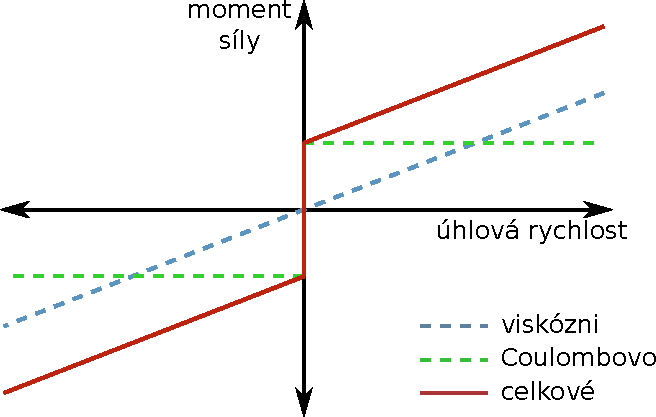
\includegraphics[width=0.65\textwidth]{treni}
\caption{Model tření os}
\label{treni_pic}
\end{figure}

Doplněním rovnice \ref{fric_eq} do dynamických rovnic robota \ref{dyn_rovnice_eq} se získají celkové rovnice dynamiky robota ve tvaru

\begin{equation}
T = M(\dot{\theta},\theta)\ddot{\theta} + C(\dot{\theta},\theta)\dot{\theta} + G(\theta) + F_v\dot{\theta} + F_csign(\dot{\theta})
\label{celkova_dyn_rovnice_eq}
\end{equation}

kde

\begin{description}
\item[$F_v$] je vektor koeficientů viskózního tření v jednotlivých osách
\item[$F_c$] je vektor koeficientů Coulombova suchého tření v jednotlivých osách
\end{description}

\section{Elektrický výkon}
\label{el_vykon_ch}
Výkon je obecně definován jako práce vykonaná za jednotku času a platí rovnice

\begin{equation}
P = \frac{W}{t}
\end{equation}

Protože v tomto případě se jedná o elektrickou práci, je tato práce definovaná jako celkový náboj $q$ přenesený mezi dvěma místy s napětím $u$. Platí tedy vztah

\begin{equation}
P = \frac{uq}{t}
\end{equation}

Pro okamžitý výkon je poté možné tento vzorec upravit na

\begin{equation}
p(t) = u(t)\frac{dq}{dt} = u(t)i(t)
\end{equation}

\subsection{Elektrický výkon v třífázové soustavě}

V případě harmonického střídavého napětí a proudu platí

\begin{equation}
\begin{split}
u\big(t\big) = U_m cos\big(\omega t + \phi\big) \\
i\big(t\big) = I_m cos\big(\omega t + \phi + \psi\big)
\end{split}
\label{harm_curr_volt_eq}
\end{equation}  
kde
\begin{description}
\item[$U_m$] je maximální amplituda napětí
\item[$I_m$] je maximální amplituda proudu
\item[$\omega$] je úhlová frekvence
\item[$\phi$] je počáteční fáze proudu a napětí
\item[$\psi$] je fázový posun mezi napětím a proudem
\end{description}

Pokud je fázový posun $\psi$ mezi napětím a proudem nenulový, je potřeba rozdělit elektrický výkon na činnou a jalovou složku. Činná složka výkonu je výkon, který je přenášen ze zdroje do spotřebiče a který je schopen konat práci. Pro činnou složku výkonu platí následující vztah

\begin{equation}
P = \frac{1}{T} \int_{t_0}^{t_0 + T} p(t)dt = UI cos\phi
\label{act_power_eq}
\end{equation}  

kde $U$ je efektivní hodnota napětí a $I$ je efektivní hodnota proudu.

Jalová složka výkonu je část výkonu, která je spotřebičem vracená zpět do zdroje a ve spotřebiči tedy žádnou práci nevykonává.

V případě třífázové soustavy je její celkový výkon roven součtu výkonů v jednotlivých fázích. Platí tedy

\begin{equation}
P = P_U + P_V + P_W
\label{3ph_power_eq}
\end{equation}  

kde $U,V,W$ jsou jednotlivé fáze v třífázové soustavě.

\subsection{Elektrický výkon synchronního motoru}

V případě výpočtu výkonu elektrického motoru je potřeba vytvořit model jeho vinutí. Synchronní motor s permanentními magnety je možné zjednodušeně modelovat jako stejnosměrný (DC) motor. Jeho elektrické schéma je na obrázku \ref{schema_motoru_pic}.  

\begin{figure}[ht]
\includegraphics[width=0.55\textwidth]{obvod_motoru}
\caption{Elektrické schéma vinutí synchronního motoru.}
\label{schema_motoru_pic}
\end{figure}

$R$ je vnitřní elektrický odpor vinutí a $L$ je jeho indukčnost. Tyto hodnoty jsou zpravidla udávány v datasheetech k motorům.

Pro okamžité napětí $u(t)$ ze schématu platí 

\begin{equation}
u(t) = i(t)R + L\frac{di(t)}{dt}
\label{motor_voltage_eq}
\end{equation}  

Okamžitý elektrický výkon motoru je poté možné z měření okamžité efektivní hodnoty proudu vypočítat jako
 
\begin{equation}
p(t) = i(t)u(t) = i(t)\left(i(t)R + L\frac{di(t)}{dt}\right)
\label{motor_power_eq}
\end{equation} 

Celkový okamžitý elektrický výkon při pohybu robota je poté dán jako součet okamžitých výkonů na všech jeho motorech
\begin{equation}
P(t) = \sum_{i=1}^{n} p_i(t)
\label{robot_motor_power_eq}
\end{equation} 
kde $n$ je počet motorů.

\section{Solver ReDySim}

Pro usnadnění odvození soustavy rovnic pro robota o 6 stupních volnosti a pro případnou standardizaci metody pro použití i pro jiné typy robotů byl použit skript pro matematický nástroj MATLAB využívající solver Recursive Dynamic Simulator (ReDySim)\cite{redysim}. Tento nástroj byl vyvinut na univerzitě v Dillí a je bezplatně k dispozici ke stažení a použití v MATLABu. Je schopen generovat rovnice pro libovolný počet os a to jak pro rotační, tak lineární osy. 

Jeho vstupními parametry jsou modifikované DH (Denavit-Hartenbergovy) parametry robota a dynamické parametry s numerickými nebo symbolickými hodnotami. Výstupem je poté skript pro MATLAB s vygenerovanými pohybovými rovnicemi zadaného robota.  

\section{Modifikované DH parametry robota}

Modifikované Denavit-Hartenbergovy (DH) parametry jsou parametry, pomocí nichž je možné kompletně popsat geometrii a kinematiku sériového robota. Jedná se o čtyři parametry pro každou osu robota, které definují vzájemnou polohu a konfiguraci sousedících os. 

Parametr $a_i [m]$ popisuje délku ramena $i$, $b_i [m]$ udává odsazení ramena $i$ podél osy rotace ramena $i-1$, parametr $\alpha_i [\si{\degree}]$ určuje vzájemný úhel natočení mezi osou $i+1$ a osou $i$ a poslední parametr $\theta_i [\si{\degree}]$ udává okamžitý úhel natočení osy $i$.

V tabulce č.\ref{tab_DH_kuka} je DH parametrizace robota KUKA KR5 Arc použita v nástroji ReDySim.

\begin{table}[htbp]
  \centering
  \caption{Tabulka DH parametrů KUKA KR5 Arc.}
    \begin{tabular}{c|cccccccccc}
    \multicolumn{1}{c|}{Osa} & \multicolumn{1}{c}{$a_{i} [m]$} & \multicolumn{1}{c}{$b_{i} [m]$} & \multicolumn{1}{c}{$\alpha_{i} [\si{\degree}]$} \\
    \hline
    1     &   0.18  &  0.4   &  90     &     \\
    2     &   0.6   &  0     &  180    &     \\
    3     &   0.12  &  0     &  -90    &     \\
    4     &   0     &  0.62  &  -90    &     \\
    5     &   0     &  0     &  90     &     \\
    6     &   0     &  0.115 &  0      &     \\
    \end{tabular}%
  \label{tab_DH_kuka}%
\end{table}% 

Přesné délky jednotlivých ramen a vzájemné polohy jednotlivých os robota je možné nalézt v jeho dokumentaci.

Pro vizualizaci DH parametrizace je možné použít nástroj RoboAnalyzer [\cite{roboanalyzer}], který byl vyvinut společně se solverem ReDySim pro účely vizualizace a simulace. RoboAnalyzer umožňuje simulovat jednoduché pohyby robota s až 7 osami a vykreslovat průběhy stavů jako jsou polohy, rychlosti, zrychlení a momenty sil na jednotlivých osách. Vizualizace použité DH parametrizace pro robota KUKA KR5 Arc v prostředí RoboAnalyzer je na obrázku \ref{dh_kuka_pic}.
\\
\begin{figure}[ht]
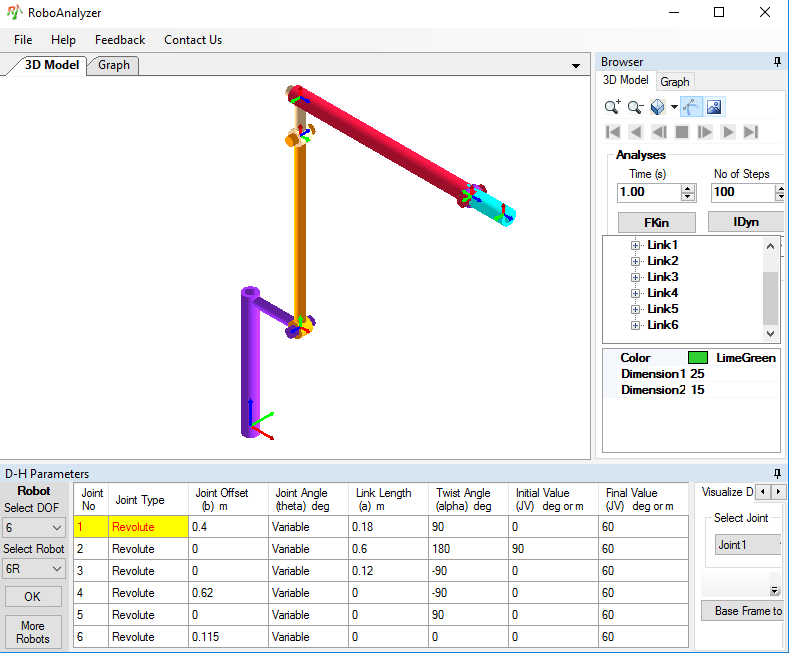
\includegraphics[width=0.95\textwidth]{pic_dh_kuka}
\caption{Vizualizace DH parametrizace robota KUKA KR5 Arc.}
\label{dh_kuka_pic}
\end{figure}

